\begin{frame}[fragile]{Introduction}
\phantomsection\label{introduction}
Jupyter Book has been rebuild from ground up using the MyST engine
{[}@Jupyter2025{]}. This allows to export content in multiple output
formats including HTML, PDF and docx. In this paper we present an
overview of the possibilities and demonstrate its working.

\begin{block}{Background}
\phantomsection\label{background}
Some background information about Jupyter Book and its features, like
exporting to multiple formats as indicated in
\{numref\}\texttt{fig-diagram}.

:::\{figure\} ../figures/diagram.* :label: fig-diagram :alt: Some figure

Some figure :::

This text should appear in all formats.

\begin{figure}
\centering
\pandocbounded{
\includegraphics[keepaspectratio]{../figures/tudelft.png}}
\caption{This picture should appear in all formats}
\end{figure}

\texttt{\{raw:latex\}\ \textbackslash{}begin\{figure\}\ \textbackslash{}centering\ \textbackslash{}only\textless{}1\textgreater{}\{\textbackslash{}includegraphics{[}width=0.5\textbackslash{}textwidth{]}\{figures/tudelft-dark.png\}\}\ \textbackslash{}caption\{This\ picture\ should\ appear\ only\ in\ beamer\}\ \textbackslash{}end\{figure\}}

This is a text that should appear in all the website, PDF and beamer
presentation.

This is a block of text that should appear only in the beamer
presentation.

\begin{figure}
\centering
\pandocbounded{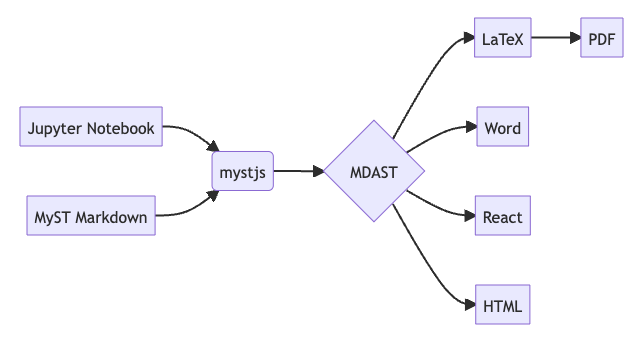
\includegraphics[keepaspectratio]{../figures/diagram.png}}
\caption{This is a picture that should appear in all the website, PDF
and beamer presentation.}
\end{figure}

\texttt{\{raw:latex\}\ \textbackslash{}begin\{figure\}\ \textbackslash{}centering\ \textbackslash{}only\textless{}1\textgreater{}\{\textbackslash{}includegraphics{[}width=0.5\textbackslash{}textwidth{]}\{figures/delft.png\}\}\ \textbackslash{}caption\{This\ is\ a\ picture\ that\ would\ appear\ only\ in\ the\ beamer\ presentation.\}\ \textbackslash{}end\{figure\}}

\begin{figure}
\centering
\pandocbounded{
\includegraphics[keepaspectratio]{../figures/tudelft.png}}
\caption{This is a picture that should appear in all the website, PDF
and beamer presentation.}
\end{figure}
\end{block}
\end{frame}
